\documentclass{article}
\usepackage{amsmath}
\usepackage{graphicx}
\begin{document}
\begin{enumerate}
    \item
        \begin{enumerate}
            \item Let $f(x) = 3\tan{x}.$ \\
                It follows that:
                \begin{equation*} \label{e1}
                \begin{split}
                    f'(x) & = 3 \sec^2{x} \\
                    f''(x) & = 6\tan{x}\sec^2{x} \\
                    f'''(x) & = 6(\sec^4{x}+2\tan^2{x}\sec^2{x}) \\
                \end{split}
                \end{equation*}
                Then, the Taylor expansion of $f(x)$ about $\dfrac{\pi}{4}$ is
                \begin{equation*} \label{e2}
                \begin{split}
                    P_3(x) & = 3 + 6(x - \dfrac{\pi}{4}) + 6(x - \dfrac{\pi}{4})^2 + 8(x - \dfrac{\pi}{4})^3 \\
                \end{split}
                \end{equation*}
            \item
                Source code can be found here: \\ \texttt{https://github.com/codeandkey/math481-iastate-sp2020} \\
                \begin{center}
                    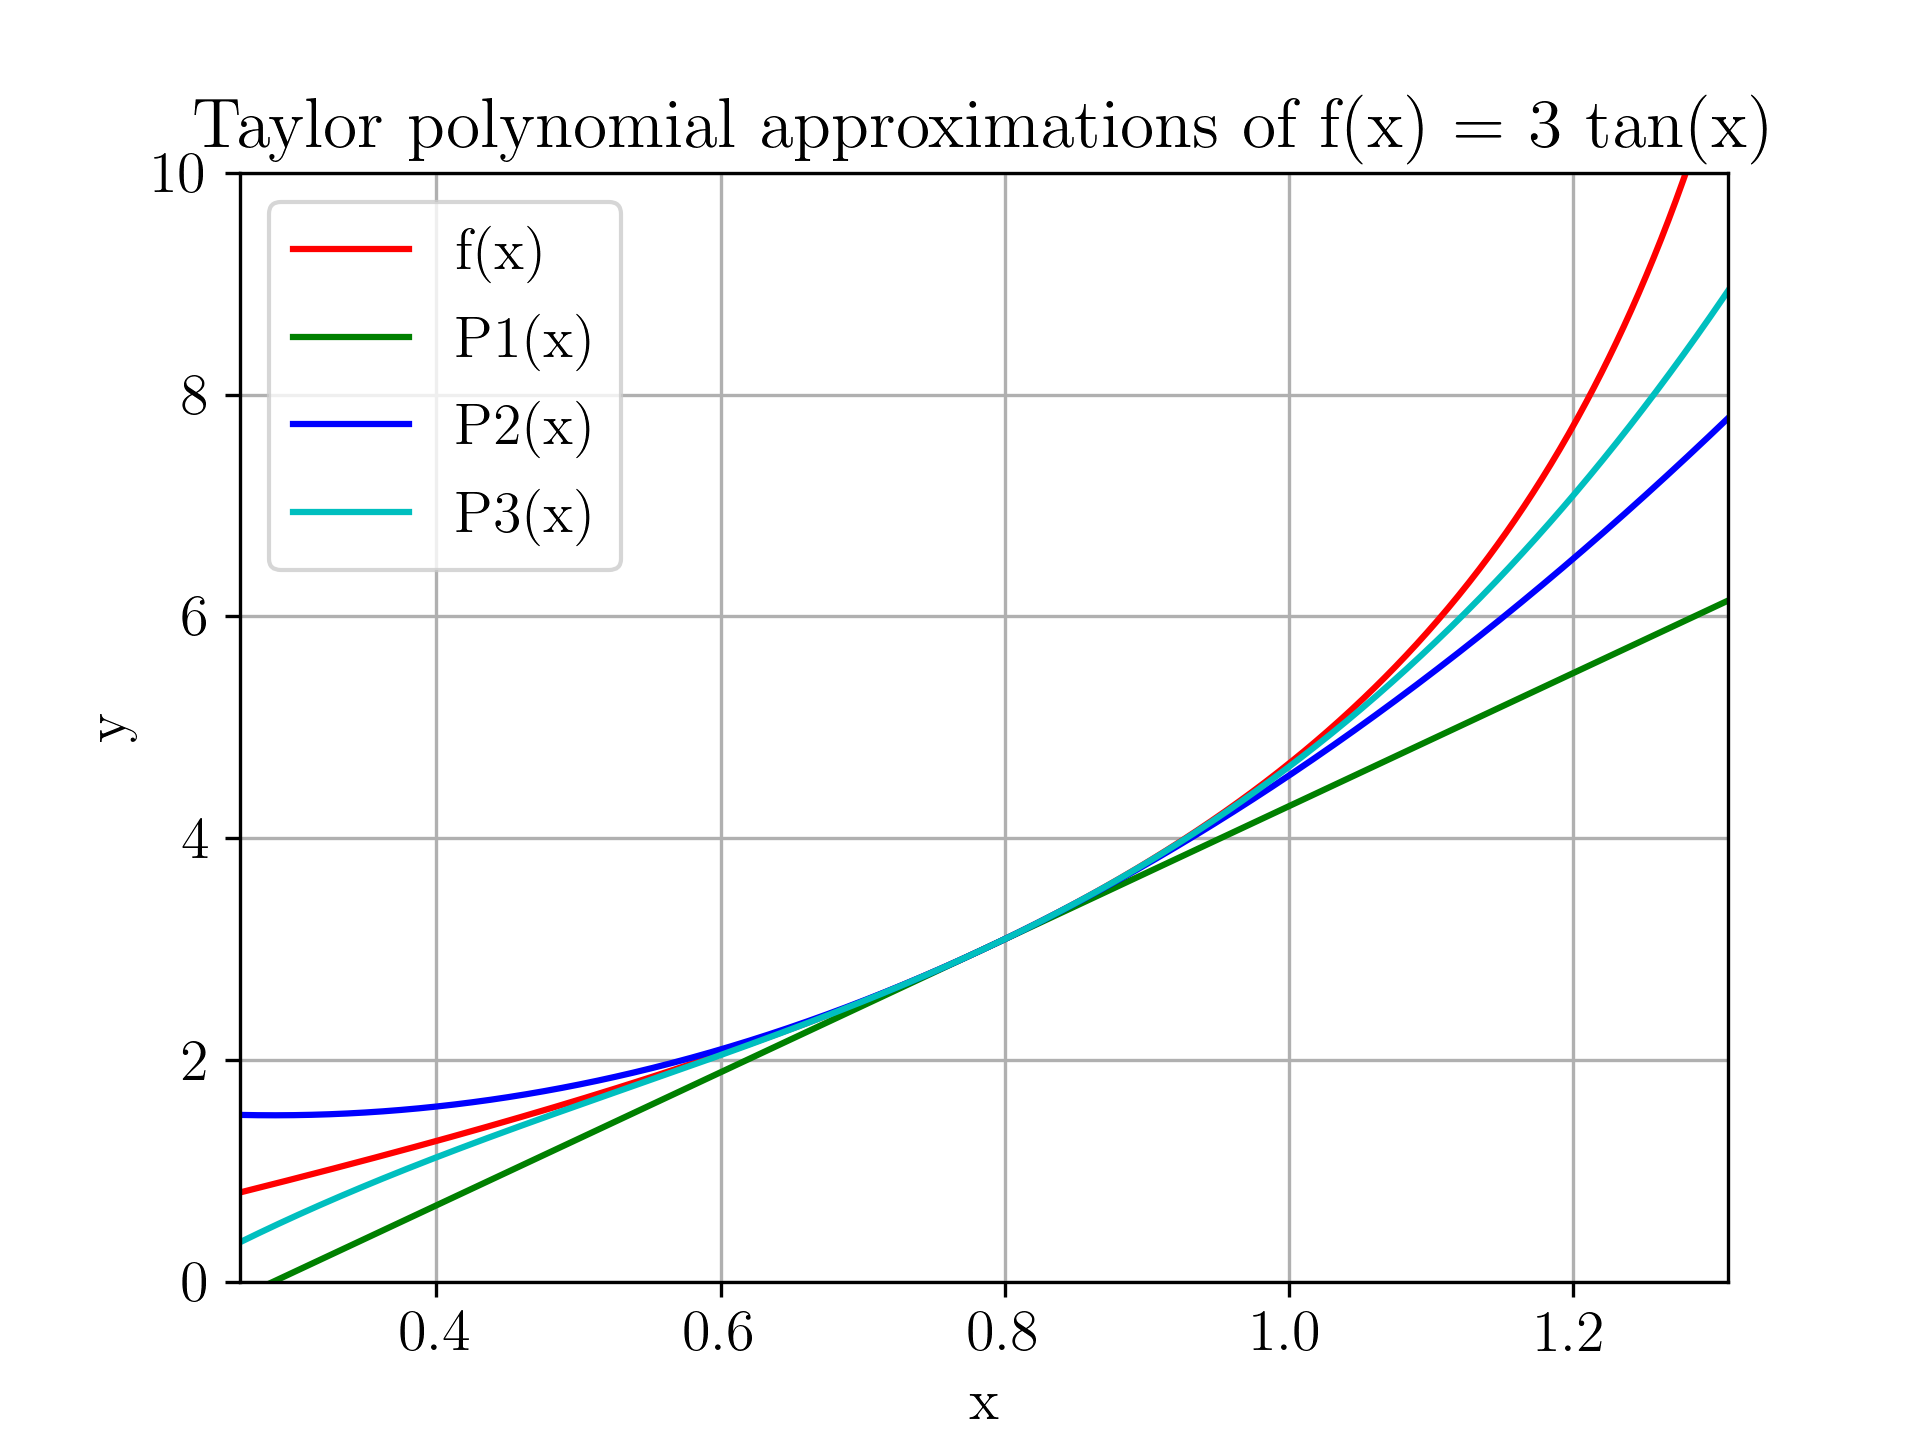
\includegraphics[width=0.75\textwidth]{q1.png}
                \end{center}
        \end{enumerate}
    \item
        Let $f(x) = \log{\left(1+xe^x\right)}$. Then, \\
        \begin{equation*}
        \begin{split}
            f'(x) & = \dfrac{e^x(x+1)}{xe^x+1} \\
            f''(x) & = \dfrac{e^x(x-e^x+2)}{(xe^x+1)^2} \\
        \end{split}
        \end{equation*}
        The Taylor polynomial coefficients are then: \\
        \begin{equation*}
        \begin{split}
            f(0) & = 0 \\
            f'(0) & = 1 \\
            f''(0) & = 1 \\
        \end{split}
        \end{equation*}
        Therefore the second-degree Taylor polynomial is $P_2(x) = x + \dfrac{x^2}{2}$. \\
        Substituting $f(x)$ back into $g(x)$ results in a simplifcation: \\
        \begin{equation*}
        \begin{split}
            g(x) & = \dfrac{f(x)}{x} \\
                 & \approx \dfrac{P_2(x)}{x} \\
                 & = \dfrac{x + \dfrac{x^2}{2}}{x} \\
                 & = 1 + \dfrac{x}{2} \\
        \end{split}
        \end{equation*}
        Here it is clear that the limit $$\lim_{x \to 0} \left(1 + \dfrac{x}{2}\right) = 1$$. \\
    \item
        \begin{enumerate}
            \item
                As all of the derivatives of $e^x$ are identical the n-th degree Taylor polynomial is as follows: \\
                \begin{equation*}
                \begin{split}
                    P_n(x) & = 1 + x + \dfrac{x^2}{2!} + \dfrac{x^3}{3!} + ... + \dfrac{x^n}{n!} \\
                \end{split}
                \end{equation*}
                The remainder $R_n(x)$ is the difference between the approximation and the exact value: \\
                \begin{equation*}
                \begin{split}
                    R_n(x) & = \left|e^x - P_n(x)\right| \\
                           & = e^x - \left(1 + x + \dfrac{x^2}{2!} + \dfrac{x^3}{3!} + ... + \dfrac{x^n}{n!}\right) \\
                \end{split}
                \end{equation*}
            \item
                Trying different values for n had the following results:
                \begin{equation*}
                \begin{split}
                    R_1(1) & \approx 0.718 \\
                    R_2(1) & \approx 0.21 \\
                    R_3(1) & \approx 0.05 \\
                    R_4(1) & \approx 0.0099 \\
                    R_5(1) & \approx 0.00161 \\
                    R_6(1) & \approx 0.0002 \\
                    R_7(1) & \approx 0.000027 \\
                    R_8(1) & \approx 0.00000305 < 10^{-5} \\
                \end{split}
                \end{equation*}
                So, $n=8$ was sufficient to bring $R_n(1)$ below $10^{-5}$. \\
            \item
                The actual error computed at $n=8$ was $0.00000305861$. \\
        \end{enumerate}
    \item
        \begin{enumerate}
            \item
                Let $f(x) = \dfrac{1}{1-x}$. \\
                The derivatives of $f(x)$ are then:
                \begin{equation*}
                \begin{split}
                    f'(x) & = \dfrac{1}{\left(1-x\right)^2} \\
                    f''(x) & = \dfrac{2}{\left(1-x\right)^3} \\
                    f'''(x) & = \dfrac{6}{\left(1-x\right)^4} \\
                    f''''(x) & = \dfrac{24}{\left(1-x\right)^5} \\
                \end{split}
                \end{equation*}
                The infinite Taylor series representation about $x = 0$ is then:
                \begin{equation*}
                \begin{split}
                    P_n(x) & = 1 + x + \dfrac{2!}{2!}x^2 + \dfrac{3!}{3!}x^3 + ... + \dfrac{n!}{n!}x^n \\
                    P_n(x) & = 1 + x + x^2 + x^3 + ... + x^n \\
                \end{split}
                \end{equation*}
            \item
                Let $x = -t^2$. Then $f(x) = \dfrac{1}{1+t^2}$, and the Taylor polynomial becomes:
                \begin{equation*}
                \begin{split}
                    P_n(x) & = 1 - t^2 + t^4 - t^6 + ... \\
                \end{split}
                \end{equation*}
            \item
                Integrating the result gives the Taylor series for $tan^{-1}(x)$ about $x=0$: \\
                $$\int_{0}^{x} \left(1 - t^2 + t^4 - t^6 + ...\right) dt = x - \dfrac{x^3}{3} + \dfrac{x^5}{5} - \dfrac{x^7}{7} + ...$$ \\
        \end{enumerate}
    \item
        \begin{enumerate}
            \item
                To solve this limit we can apply L'Hopital's rule successively: 
                \begin{equation*}
                \begin{split}
                    \lim_{h\to 0} F(h) & = \lim_{h\to 0} \dfrac{\sin{h}-h\cos{h}}{h^3} \\
                    & = \lim_{h\to 0} \dfrac{h\sin{h}}{3h^2} \\
                    & = \lim_{h\to 0} \dfrac{\sin{h} + h\cos{h}}{6h} \\
                    & = \lim_{h\to 0} \dfrac{2\cos{h} - h\sin{h}}{6} \\
                    & = \dfrac{2 - 0}{6} \\
                    & = \dfrac{1}{3} \\
                \end{split}
                \end{equation*}
            \item
                To find the rate of the convergence, the remainder can be manipulated: \\
                \begin{equation*}
                \begin{split}
                    \lim_{h\to 0} F(h) & = \lim_{h\to 0} \dfrac{\sin{h}-h\cos{h}}{h^3} = \dfrac{1}{3} \\
                    & = \lim_{h\to 0} \left|\dfrac{1}{3} - \dfrac{\sin{h}-h\cos{h}}{h^3}\right| = 0 \\
                    & \leq \left|\dfrac{h^3}{3} - \sin{h} - h\cos{h}\right| \\
                    & \leq \left|h^3\right|\\
                \end{split}
                \end{equation*}
                So, the rate of convergence is bounded from above by $O(h^3)$.
        \end{enumerate}
    \item
        \begin{enumerate}
            \item
                See the source code in the link from part 1.
            \item
                The program reported $N=4$ to be sufficiently large, with $x^N \approx 0.2575302$.
        \end{enumerate}
\end{enumerate}
\end{document}
